\documentclass[20pt]{report}
\usepackage{amsmath, amssymb,amsmath}

\usepackage[spanish, es-lcroman]{babel}  
\usepackage[spanish]{babel}
\usepackage{multicol}
\usepackage{graphicx}
\usepackage{makeidx}
\usepackage{multicol}
 \cleardoublepage
\usepackage{graphicx}
\usepackage{float}
\providecommand{\abs}[1]{\lvert#1\rvert}
\providecommand{\norm}[1]{\lVert#1\rVert}
\usepackage{listings}
\usepackage{fancybox}
\usepackage{cancel}
%\usepackage{float}
\usepackage{wrapfig}
\parindent=2.1pc
\setlength{\oddsidemargin}{0.5cm} \setlength{\evensidemargin}{0cm}
\setlength{\textwidth}{16cm} \setlength{\textheight}{23cm}
\setlength{\topmargin}{-.5cm}
\begin{document}

\begin{figure}[H]
  \scalebox{0.5}{
    
\includegraphics[scale=0.2]{1.jpg} 
    %\caption{Descripci\'on si se desea} 
    }
\end{figure}

\begin{figure}[H]
  \scalebox{0.5}{
  
    
\includegraphics[scale=0.5]{udec4.jpg} 
    %\caption{Descripci\'on si se desea} 
    }
    \centering
\end{figure}


\topmargin=-1.6cm

%%%%%%%%%%%%%%%%%%%%% ENCABEZADO %%%%%%%%%%%%%%%%%%%%%%%%%%%%%%%%

\vspace{1cm}

\noindent\rule{15cm}{.5pt}

\begin{center}
\noindent{\huge\textbf{{UNIVERSIDAD DE CONCEPCI\'ON}}}\\
\noindent{\Large\textbf{{FACULTAD DE CIENCIAS F\'ISICAS Y MATEM\'ATICAS }}}\\

{DEPARTAMENTO DE INGENIER\'IA EN MATEM\'ATICA}
\end{center}
\begin{center}
\noindent\rule{15cm}{.5pt}\\
\vspace{2cm}
\textbf{\Large{ CENTRO DE MASA POBLACIONAL DE CHILE}}\\

\Large{Sebasti\'an Moraga Scheuermann}\\

\Large{Profesor Dr. Leonardo Figueroa}\\

\end{center}
%\vspace{0.5cm} \centerline{\bf \large } 



 %\centerline{\bf \large Ingenier\'ia Civil Matem\'atica}\\
 %\centerline{\bf \large Universidad de Concepci\'on}
%%%%%%%%%%%%%%%%%%%%%%%%%%%%%%%%%%%%%%%%%%%%%%%%%%%%%%%%%%%%%%%%%
 \vspace{.2cm}
  \noindent
%%%%%%%%%%%%%%%%%%%%%%%%%%%%%%%%%%%%%%%%%%%%%%%%%%%%%%%%%%%%%%%%%
\begin{itemize}
\item [\bf ]{\bf    }
\topmargin=-1.6cm


\end{itemize}
\topmargin=-1.6cm
\vspace{3cm}
\noindent 



%\rule{16cm}{.5pt} 



\pagebreak


 \tableofcontents % indice de contenidos


\chapter{Introducci\'on}\label{cap.introduccion}

\pagenumbering{arabic} % para empezar la numeraci\'on con n\'umeros
En los tiempos actuales es m\'as  necesario  que nunca poder resolver problemas de modelaci\'on, ya que estos pueden  ser una aproximaci\'on a la realidad que f\'acilmente pueden validar un modelo y al mismo tiempo ahorrar una cantidad de capital considerable para quienes opten por este camino. 
\\
El siguiente texto tiene como inter\'es principal mostrar un camino  para la obtenci\'on del centro poblaci\'on de un pa\'is en general. EL m\'etodo usado para la obtenci\'on es sencillo y f\'acil de explicar, la parte te\'orica es m\'as sencilla que la  implementaci\'on, sin embargo, se requiere de conocimiento matem\'atico para su construcci\'on. 
\\
Luego de su construcci\'on te\'orica se   aplica el procedimiento  para  obtener el centro de masa poblaci\'on de  Chile.
\\
\\
Se construy\'o el programa basado  en el lenguaje de programaci\'on Python.

\pagebreak



\chapter{Enunciado }\label{cap.introduccion}
\section{ Inter\'es}
\begin{itemize}
\item Sea $\Omega$ la superficie de la Rep\'ublica de Chile y sea $\rho$ una aproximaci\'on de la funci\'on densidad-humana definida sobre $\Omega$. Compute el centro de masa de $\rho$ (que es un punto bajo la superficie del planeta Tierra) y su proyecci\'on sobre la superficie del planeta Tierra.
\\


\begin{figure}[H]
\begin{center}
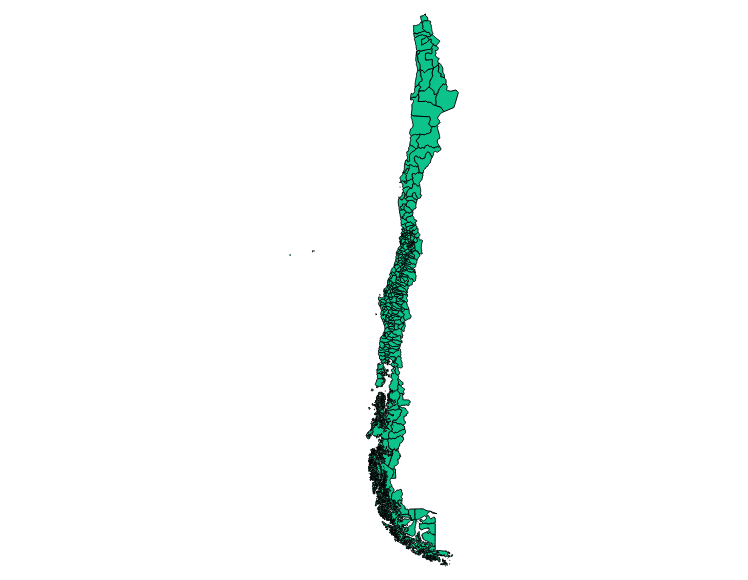
\includegraphics[width=10cm, height=10cm]{chile.png}
\vspace{-0.5cm} %Espacio vertical negativo para pegar mas el caption de la figura a la propia figura
\caption{Chile}
\label{Label para referencia}
\end{center}
\end{figure}
\pagebreak
\label{cap.introduccion}\section{Introducci\'on}

A modo de introducci\'on el formato ESRI Shapefile (SHP) es un formato de archivo inform\'atico propietario de datos espaciales desarrollado por la compa\~n\'ia ESRI, datos que contiene  lo necesario para obtener la forma de un lugar en el espacio y sus coordenadas. Se obtuvieron los archivos necesarios para el problema de  www.bcn.cl  y en Wikipedia. Sin embargo este archivo division\_comunal.shp no contiene la cantidad de habitantes   por comuna. Por lo cual se debi\'o crear un archivo H.py que contiene  dichos datos. \\

\begin{figure}[H]
\begin{center}
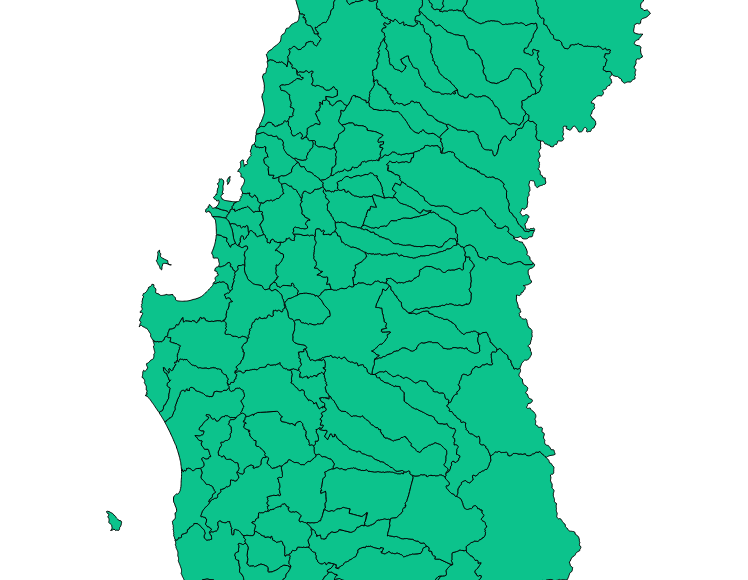
\includegraphics[width=10cm, height=10cm]{biobio.png}
\vspace{-0.5cm} %Espacio vertical negativo para pegar mas el caption de la figura a la propia figura
\caption{Regi\'on B\'io - B\'io}
\label{Label para referencia}
\end{center}
\end{figure}


\label{cap.introduccion}\section{Formulaci\'on Matem\'atica }
En primer lugar en el programa ser\'a realizado en Python 2.17, y se usar\'an los packages GDAL y Scipy, estos son necesarios para poder tener las coordenadas en  $\phi,\theta$ las cuales  conocemos y podemos usar para resolver las integrales. Esto es debido a que computar las integrales  con las coordenadas en las que vienen el .shp no es posible, pues estas no son coordenadas cartesianas.
\\
Como es de esperarse la alimentaci\'on de las integrales es $\phi$ (Longitud) y $\theta$ (Colatitud)
\\
\\

Dada $D$ una regi\'on de v\'ertices $(\varphi_0, \theta_0)$, $(\varphi_1, \theta_1)$, $(\varphi_2, \theta_2)$,...,$(\varphi_p, \theta_p)$ dados en sentido antihorario; esto es,
\begin{equation}\label{T}
D = \left\{ \sum_{i=0}^p t_i (\varphi_i, \theta_i) \mid 0 \leq t_0, t_1, t_2,...,t_p \leq 1 \ \wedge \ t_0+t_1+t_2+...+t_p=1 \right\}.
\end{equation}
Deseamos computar las integrales

\begin{equation}\label{I1}
I_{D,x} := \int_D x(\varphi, \theta) \rho_D(\varphi,\theta) dS(\varphi, \theta) 
\end{equation}
\begin{equation}\label{I1}
I_{D,y} := \int_D y(\varphi, \theta) \rho_D(\varphi,\theta) dS(\varphi, \theta) 
\end{equation}
\begin{equation}\label{I1}
I_{D,z} := \int_D z(\varphi, \theta) \rho_D(\varphi,\theta) dS(\varphi, \theta) 
\end{equation}
Para evitar calcular directamente estas integrales usaremos el teorema de la divergencia, para ello primero expresaremos cada una de estas integrales en  sus coordenadas $(\varphi, \theta)$
\\
Usando el hecho que:
\[x=R\sin(\theta)\cos(\varphi),y=R\sin(\theta)\sin(\varphi),z=R\cos(\theta) \]
\begin{equation}\label{I1}
I_{D,x} := \int_D  R^2\sin^2(\theta)\cos(\varphi) dS(\varphi, \theta) 
\end{equation}
\begin{equation}\label{I1}
I_{D,y} := \int_D R^2\sin^2(\theta)\sin(\varphi) \rho_D(\varphi,\theta) dS(\varphi, \theta) 
\end{equation}
\begin{equation}\label{I1}
I_{D,z} := \int_D R^2\cos(\theta)\sin(\theta) \rho_D(\varphi,\theta) dS(\varphi, \theta) 
\end{equation}
Para ocupar el teorema de la divergencia primero encontraremos antidiergencia para cada uno de los integrandos anteriores, lo cual no es dificil. Dado que la densidad en cada regi\'on D es constante este termino podemos dejarlo afuera, al igual que el Radio de la tierra R.
\begin{equation}\label{F}
F_x(\varphi, \theta) = \begin{bmatrix}
\sin^2(\theta)\sin(\phi)\\[2ex]
0
\end{bmatrix}
\end{equation}
%
\begin{equation}\label{F}
F_y(\varphi, \theta) = \frac{1}{2}\begin{bmatrix}
-\cos(\phi)\sin^2(\theta) \\[2ex]
0
\end{bmatrix}
\end{equation}
\begin{equation}\label{F}
F_z(\varphi, \theta) = \frac{1}{4}\begin{bmatrix}
0\\[2ex]
-cos(2\theta)
\end{bmatrix}
\end{equation}
satisface


\begin{equation*}
\operatorname{div}(F_x)(\varphi,\theta)
= \frac{\partial F_{x1}(\varphi, \theta)}{\partial \varphi} + \frac{\partial F_{x2}(\varphi, \theta)}{\partial \theta}
= \cos(\varphi) \sen(\theta)^2.
\end{equation*}

\begin{equation*}
\operatorname{div}(F_y)(\varphi,\theta)
= \frac{\partial F_{y1}(\varphi, \theta)}{\partial \varphi} + \frac{\partial F_{y2}(\varphi, \theta)}{\partial \theta}
= \sin(\varphi) \sen(\theta)^2.
\end{equation*}
\begin{equation*}
\operatorname{div}(F_z)(\varphi,\theta)
= \frac{\partial F_{z1}(\varphi, \theta)}{\partial \varphi} + \frac{\partial F_{z2}(\varphi, \theta)}{\partial \theta}
= \sin(\theta)\cos(\theta)
\end{equation*}


\begin{equation}\label{I3}
I_{D,x} = \int_{\partial D} F(\varphi, \theta) \cdot \nu_D(\varphi,\theta) dl(\varphi, \theta)
= \sum_{i=0}^{p-1} \int_{E_i} F(\varphi, \theta) \cdot \nu_D(\varphi,\theta) dl(\varphi, \theta),
\end{equation}
%
Donde $\nu_D$ es el vector unitario exterior normal a $D$ definido sobre $\partial D$, $l$ es la medida lineal sobre $\partial D$ y para cada $i \in \{0, 1, 2,..p-1\}$, $E_i$ es el segmento que une a $(\varphi_i, \theta_i)$ con $(\varphi_{i+1}, \theta_{i+1})$
\begin{equation}\label{Ei}
(\forall\,i\in\{0,1,2,...,p-1\}) \quad E_i = \left\{ (1-s) (\varphi_i, \theta_i) + s (\varphi_{i+1}, \theta_{i+1}) \mid 0 \leq s \leq 1 \right\}.
\end{equation}
%
Ahora, usando la parametrizaci\'on de $E_i$ sugerida por \eqref{Ei}, las \'ultimas integrales en \eqref{I3} se pueden escribir en la forma

\begin{multline}\label{lineIntegrals}
\int_{E_i} F(\varphi, \theta) \cdot \nu_T(\varphi,\theta) d l(\varphi, \theta)\\
= \int_0^1 F\big( (1-s) (\varphi_i, \theta_i) + s (\varphi_{i+1}, \theta_{i+1}) \big) \cdot \left[ \frac{1}{\abs{E_i}} \begin{bmatrix} 0 & 1\\-1 & 0\end{bmatrix} \begin{bmatrix} \varphi_{i+1}-\varphi_i \\ \theta_{i+1} - \theta_i \end{bmatrix} \right] \abs{E_i} d s\\
= \int_0^1 F\big( (1-s) (\varphi_i, \theta_i) + s (\varphi_{i+1}, \theta_{i+1}) \big) \cdot \begin{bmatrix} \theta_{i+1}-\theta_i\\ -(\varphi_{i+1} - \varphi_i) \end{bmatrix} d s.
\end{multline}
 
Haciendo esto para $F_x,F_y,F_z$ logramos programar f\'acilmente en Python una rutina para que haga esto para puntos en el mapeo.
\\
Es decir podemos computar lo siguiente en una rutina de Python
\begin{equation}
I_{D,x}= \sum_{i=0}^{p-1}\int_{0}^1 -\sin^2(\theta_i - s(\theta_i - \theta_{i+1})) \sin(\phi_i - s(\phi_i - \phi_{i+1}))(\theta_i - \theta_{i+1}) ds
\end{equation}
\begin{equation}
I_{D,y}= \sum_{i=0}^{p-1}\int_{0}^1 \cos(\phi_i - s(\phi_i - \phi_{i+1}))sin^2(\theta_i - s(\theta_i - \theta_{i+1}))(\theta_i - \theta_{i+1}) ds
\end{equation}

\begin{equation}
I_{D,z}= \sum_{i=0}^{p-1} \dfrac{sin(2\theta_i - 2s(\theta_i - \theta_{i+1})(\phi_i - \phi_{i+1})}{8(\theta_i - \theta_{i+1})}|_{0}^1
\end{equation}


Con esto en mente podemos calcular cada integral en un Poligono $D$, por simple notaci\'on designaremos $C$ como cada comuna.
\\
De esta manera y siguiendo la misma notaci\'on.
\begin{equation}
\int_{\Omega} \overline{x}\rho(\overline{x}) dS(\overline{x})=\sum_{C} R^2  \lbrace \rho_{C} \sum_{D} I_{D,x} + I_{D,y}+ I_{D,z} \rbrace 
\end{equation}
\begin{equation}
\int_{\Omega} \rho(\overline{x}) dS(\overline{x})=p
\end{equation}
Con $p$ la poblaci\'on completa de Chile.
De manera an\'aloga se calcul\'o la densidad para cada  comuna. 
\begin{equation}
\rho_{C}= \dfrac{H_C}{ \int_{C} dS(\overline{x}) \hspace{0.1cm} }  
\end{equation}
Con $H_C$ es la Poblaci\'on en cada comuna.\\

As\'i el punto que queremos obtener es el centro de masa poblacional $CM$
$${CM}=\dfrac{\int_{\Omega} \overline{x}\rho(\overline{x}) dS(\overline{x})}{\int_{\Omega} \rho(\overline{x}) dS(\overline{x})}$$
\pagebreak

\label{cap.introduccion}\section{Resultados num\'ericos} 
Programando este m\'etodo en Python 2.17 se lograron los siguientes resultados num\'ericos. 
\[Longitud=-71.248133308597588 ^\circ \]
\[Latitud=-34.137708515814154^\circ \]
El programa demora $7$ minutos con $20.3$ segundos en un computador Intel(R) Core(TM) i$5$-$4200$M CPU @ $2.50$ GHz de $8,00$Gb RAM
\begin{figure}[H]
\begin{center}
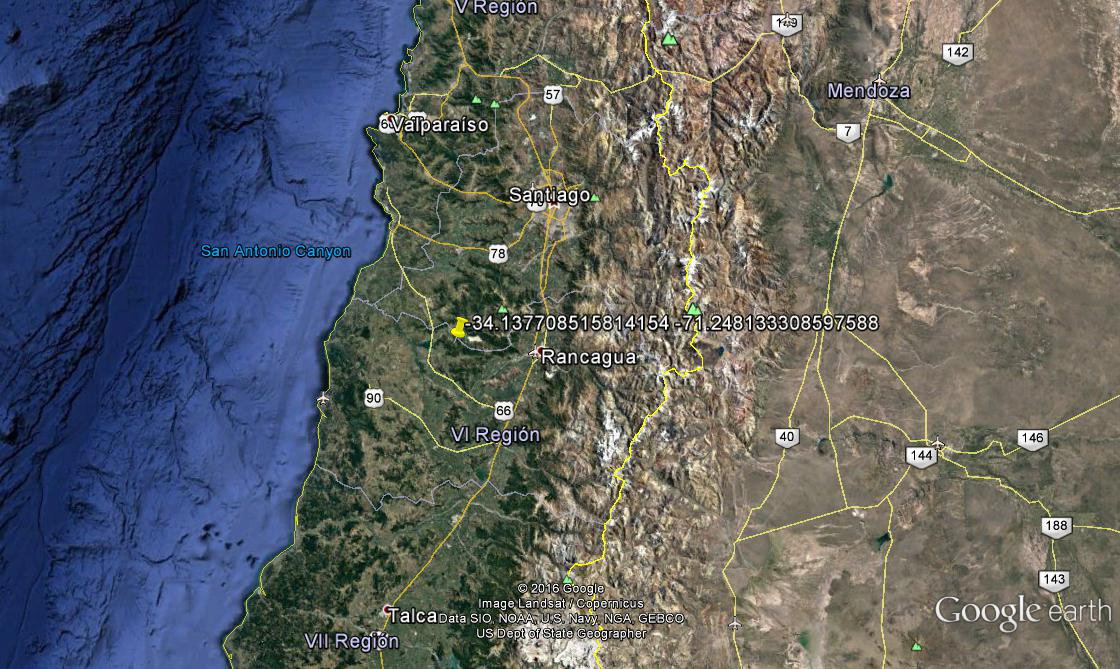
\includegraphics[width=15cm, height=10cm]{centro2.png}
\vspace{-0.5cm} %Espacio vertical negativo para pegar mas el caption de la figura a la propia figura
\caption{Centro poblaciona de Chile, altura=$521.65$km}
\label{Label para referencia}
\end{center}
\end{figure}
\pagebreak
A modo de  respaldo para el m\'etodo se realiz\'o un test en el mismo programa PROYECTOFINAL.py, una completa evaluaci\'on de las integrales y el c\'alculo de cada centro de masa para cada poligono, esto valida nuestro m\'etodo para poder computar las integrales antes mencionadas. Se revis\'o cada una de las $346$ comunas, pero solo expondremos tres casos en este informe. Las dem\'as se pueden verificar haciendo correr el programa pues generar\'a autom\'aticamente las im\'agenes. 
\begin{figure}[H]
\begin{center}
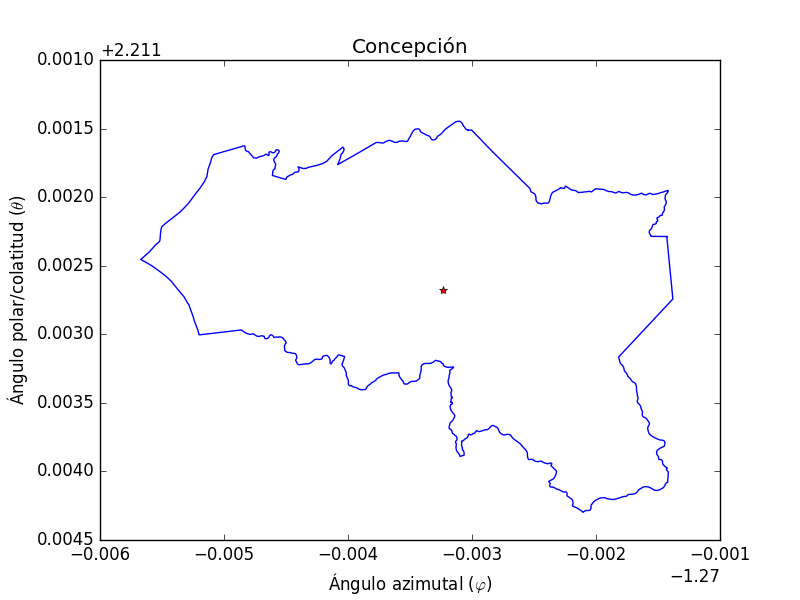
\includegraphics[width=15cm, height=10cm]{FiguraCentroDeMasaComunal141.png}
\vspace{-0.5cm} %Espacio vertical negativo para pegar mas el caption de la figura a la propia figura
\caption{Concepci\'on y su centro de masa.}
\label{Label para referencia}
\end{center}
\end{figure}
\begin{figure}[H]
\begin{center}
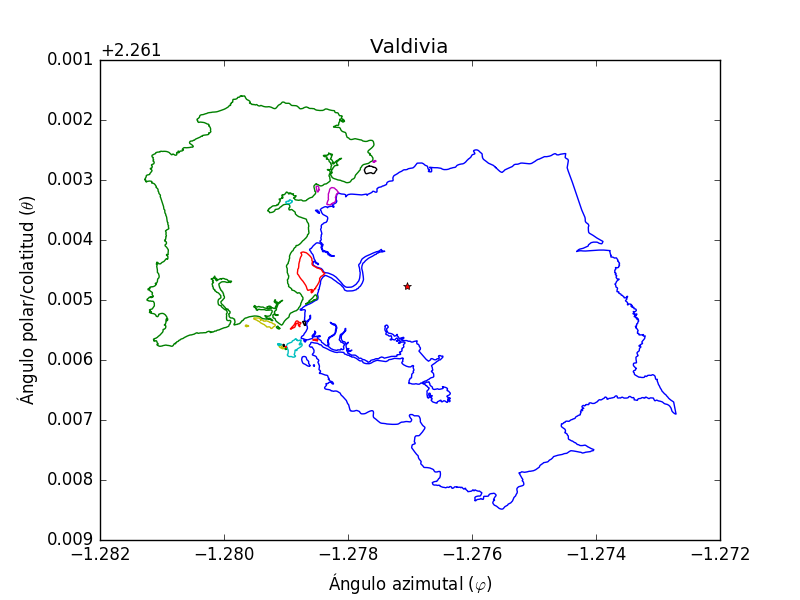
\includegraphics[width=15cm, height=10cm]{FiguraCentroDeMasaComunal238.png}
\vspace{-0.5cm} %Espacio vertical negativo para pegar mas el caption de la figura a la propia figura
\caption{Valdivia y su centro de masa.}
\label{Label para referencia}
\end{center}
\end{figure}
\begin{figure}[H]
\begin{center}
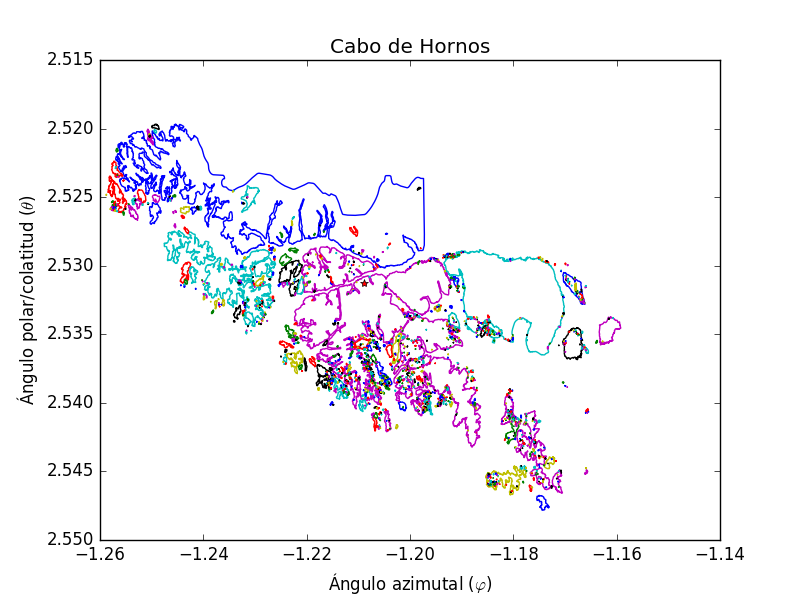
\includegraphics[width=15cm, height=10cm]{FiguraCentroDeMasaComunal324.png}
\vspace{-0.5cm} %Espacio vertical negativo para pegar mas el caption de la figura a la propia figura
\caption{Cabo de Hornos y su centro de masa.}
\label{Label para referencia}
\end{center}
\end{figure}
\pagebreak

\section{Conclusiones}
El resultado num\'erico es como se esperaba, el tiempo  en que demora el programa en realizar todos los procesos sigue siendo bastante, sin embargo  razonable. El mayor tiempo se consume en  integrar con la rutina QUAD de Python  las integrales $I_{D,x}$ e $I_{D,y}$ ya que las del \'area y $I_{D,z}$ fueron calculadas de manera exacta.\\

Se est\'a trabajando en  realizar el mismo computo pero en Geod\'esicas, y as\'i obtener un  menor tiempo de c\'alculo para el programa.\\
\\

Tenemos otra  muestra de este punto en la Figura $2.3$  mucho m\'as cercano, a una altura de $26.67$km, donde se puede ver ciudades cercanas y  el parque nacional Las Palmas de Cocal\'an.

\begin{figure}[H]
\begin{center}
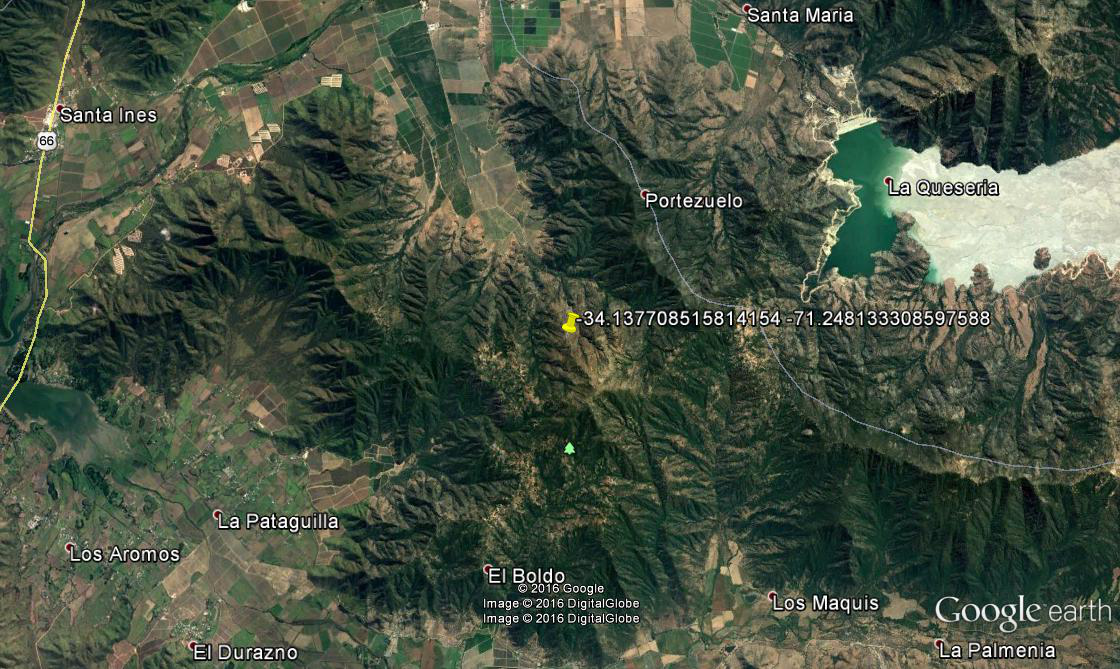
\includegraphics[width=15cm, height=10cm]{centro.png}
\vspace{-0.5cm} %Espacio vertical negativo para pegar mas el caption de la figura a la propia figura
\caption{Centro poblaciona de Chile, altura=$21.67$km}
\label{Label para referencia}
\end{center}
\end{figure}
\pagebreak


\section{Bibliografia}
\item http:\textbackslash \textbackslash  www.bcn.cl \textbackslash siit\textbackslash mapas\_ vectoriales\textbackslash index\_ html
\item https:\textbackslash \textbackslash es.wikipedia.org\textbackslash wiki\textbackslash Coordenadas\_ esf\'ericas
\item https:\textbackslash \textbackslash www.python.org\textbackslash
\end{itemize}
\end{document}

